\documentclass{standalone}
%<--------------------------------------------------------------------------->%
%%% TikZ %%%
\usepackage{tikz}
\usetikzlibrary{fit}
% \usetikzlibrary{calc}
% \usetikzlibrary{angles,quotes}
% \usetikzlibrary{intersections,topaths}
% \usetikzlibrary{decorations.markings}
%<--------------------------------------------------------------------------->%

\begin{document}

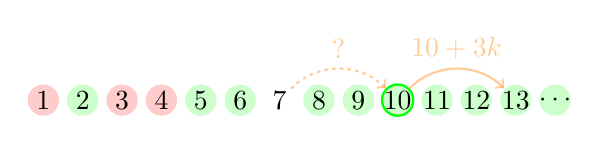
\begin{tikzpicture}[scale=1/2,thick,line cap=round]
	\tikzstyle{jiao}=[inner sep=0.4em,fill=none,circle];
	%% status
	\node[jiao,fill=red!20]   (A) at (1,0)  {};
	\node[jiao,fill=green!20] (B) at (2,0)  {};
	\node[jiao,fill=red!20]   (C) at (3,0)  {};
	\node[jiao,fill=red!20]   (D) at (4,0)  {};
	\node[jiao,fill=green!20] (E) at (5,0)  {};
	\node[jiao,fill=green!20] (F) at (6,0)  {};
	\node[jiao]               (G) at (7,0)  {};
	\node[jiao,fill=green!20] (H) at (8,0)  {};
	\node[jiao,fill=green!20] (I) at (9,0)  {};
	\node[jiao,fill=green!20,draw=green] (J) at (10,0) {};
	\node[jiao,fill=green!20] (K) at (11,0) {};
	\node[jiao,fill=green!20] (L) at (12,0) {};
	\node[jiao,fill=green!20] (M) at (13,0) {};
	\node[jiao,fill=green!20] (N) at (14,0) {};
	%% numbers
	\node[inner sep=0.1em] at (1,0)  {1};
	\node[inner sep=0.1em] at (2,0)  {2};
	\node[inner sep=0.1em] at (3,0)  {3};
	\node[inner sep=0.1em] at (4,0)  {4};
	\node[inner sep=0.1em] at (5,0)  {5};
	\node[inner sep=0.1em] at (6,0)  {6};
	\node[inner sep=0.1em] at (7,0)  {7};
	\node[inner sep=0.1em] at (8,0)  {8};
	\node[inner sep=0.1em] at (9,0)  {9};
	\node[inner sep=0.1em] at (10,0) {10};
	\node[inner sep=0.1em] at (11,0) {11};
	\node[inner sep=0.1em] at (12,0) {12};
	\node[inner sep=0.1em] at (13,0) {13};
	\node[inner sep=0.1em] at (14,0) {$\cdots$};
	%% connections
	% \draw[opacity=0.4] (B) edge[bend left=45,->] node[pos=0.5,above]{$2+3k$} (E);
	% \draw[opacity=0.4] (E) edge[bend left=45,->] (H);
	% \draw[opacity=0.4] (H) edge[bend left=45,->] (K);
	% \draw[opacity=0.4] (F) edge[bend right=45,->,blue] node[pos=0.5,below]{$6+3k$} (I);
	% \draw[opacity=0.4] (I) edge[bend right=45,->,blue] (L);
	\draw[opacity=0.4] (G) edge[bend left=45,->,orange,dotted] node[above]{?} (J);
	\draw[opacity=0.4] (J) edge[bend left=45,->,orange] node[pos=0.5,above]{$10+3k$} (M);
	%% fitting
	% \node[inner sep=0.1em,draw,thin,densely dotted,opacity=0.8,rounded corners,rectangle,fit=(H) (I) (J)] {};
\end{tikzpicture}

\end{document}
